% Created 2016-09-27 mar 12:19
\documentclass[captions=tableheading]{scrartcl}
\usepackage[utf8]{inputenc}
\usepackage[T1]{fontenc}
\usepackage{fixltx2e}
\usepackage{graphicx}
\usepackage{longtable}
\usepackage{float}
\usepackage{wrapfig}
\usepackage{rotating}
\usepackage[normalem]{ulem}
\usepackage{amsmath}
\usepackage{textcomp}
\usepackage{marvosym}
\usepackage{wasysym}
\usepackage{amssymb}
\usepackage{hyperref}
\tolerance=1000
\usepackage{tikz,pgf,pgfplots,tikz-qtree,scalefnt}
\usepackage[margin=25mm]{geometry}
\usepackage[parfill]{parskip}
\usepackage{graphicx}
\renewcommand{\theenumi}{\alph{enumi}}
\author{Kjartan Halvorsen}
\date{\today}
\title{Lathund för analys av IMU-data för mörkerstudien}
\hypersetup{
  pdfkeywords={},
  pdfsubject={},
  pdfcreator={Emacs 24.5.1 (Org mode 8.2.10)}}
\begin{document}

\maketitle
\tableofcontents


\section{Översikt}
\label{sec-1}
Data från IMU'erna delas upp och märks med försöksperson nummer och typ av försök (monokulär, binokulär, etc), för att därefter läggas in i en databas på formatet hdf5. Detta det smidigt att plocka fram och bearbeta delar av data. Första steget är därför att förbereda data för att läggas in i databasen. Därefter finns det ett antal olika kommandon för att göra beräkningar på data.
\section{Program att installera}
\label{sec-2}
\subsection{Python}
\label{sec-2-1}
\begin{itemize}
\item \href{https://code.google.com/p/pythonxy/wiki/Downloads?tm\%3D2}{Python(x,y) scientific python}
\item Ladda ner installationsprogrammet (drygt 600Mb).
\item Öppna installeraren. Acceptera licensen
\item I dialogen där du väljer vad som ska installeras, så välj allt genom att klicka i check-boxen framför Python och framför Other

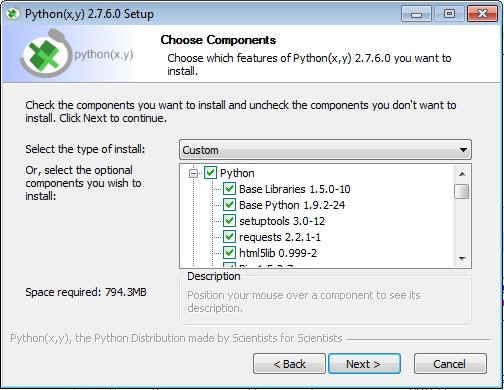
\includegraphics[width=0.4\linewidth]{xyinstall}
\end{itemize}
\subsection{Python-kod för att bearbeta imudata}
\label{sec-2-2}
\begin{itemize}
\item \href{https://github.com/alfkjartan/nvgimu/archive/master.zip}{nvgimu zip-fil}
\item Extrahera filerna till valfri plats på hårddisken.
\item Öppna kommandofönstret (\emph{command prompt})
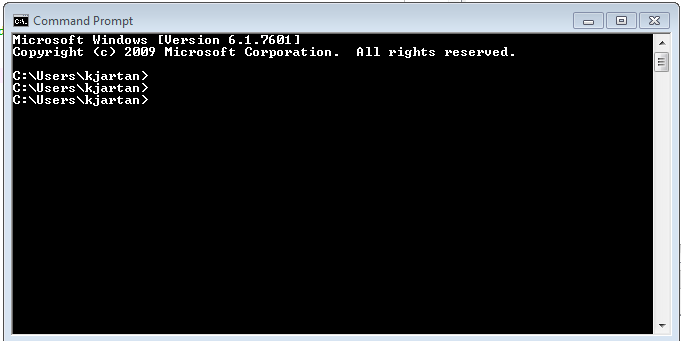
\includegraphics[width=0.4\linewidth]{commandprompt1}
\item Gör \texttt{cd} (change directory) till katalogen \texttt{nvgimu} som du precis extraherat.
\item Installera programmet genom att ange \texttt{c:\textbackslash{}blabla\textbackslash{}nvgimu>python setup.py build}, och därefter \texttt{c:\textbackslash{}blabla\textbackslash{}nvgimu>python setup.py install}.
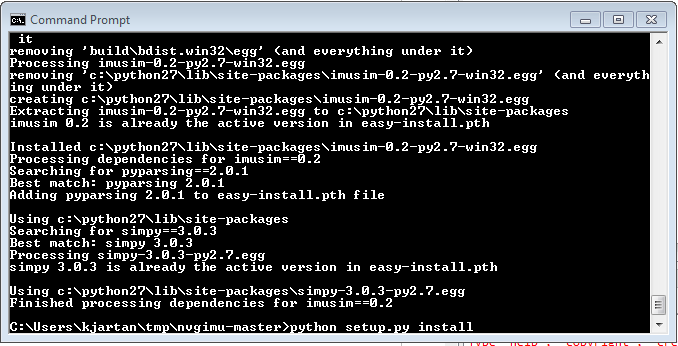
\includegraphics[width=0.4\linewidth]{commandprompt2}
\end{itemize}
\subsection{Tidigare data}
\label{sec-2-3}
Data från försök i labbet 2012 finns samlade i en stor hdf5-fil. Denna kan laddas ner här:
\href{https://dl.dropboxusercontent.com/u/10481140/nvg201209.hdf5}{nvg data hdf-format}
Spara filen på valfri plats på datorn. Notera platsen, då du kommer behöva den sedan.
\section{Öppna programmet}
\label{sec-3}
\begin{itemize}
\item Öppna Python(x,y) start-dialogen. Den finns under Start->Alla program->Python(x,y).
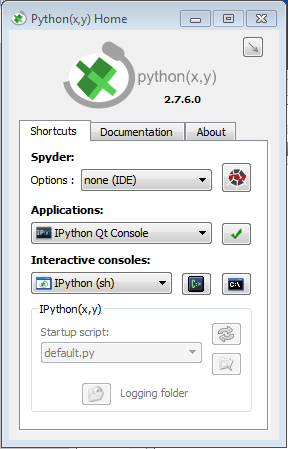
\includegraphics[width=0.3\linewidth]{xystartdialog}
\item Starta Spyder
\item Spyder är ett program för att arbeta med python. Det påminner en del om Matlab.
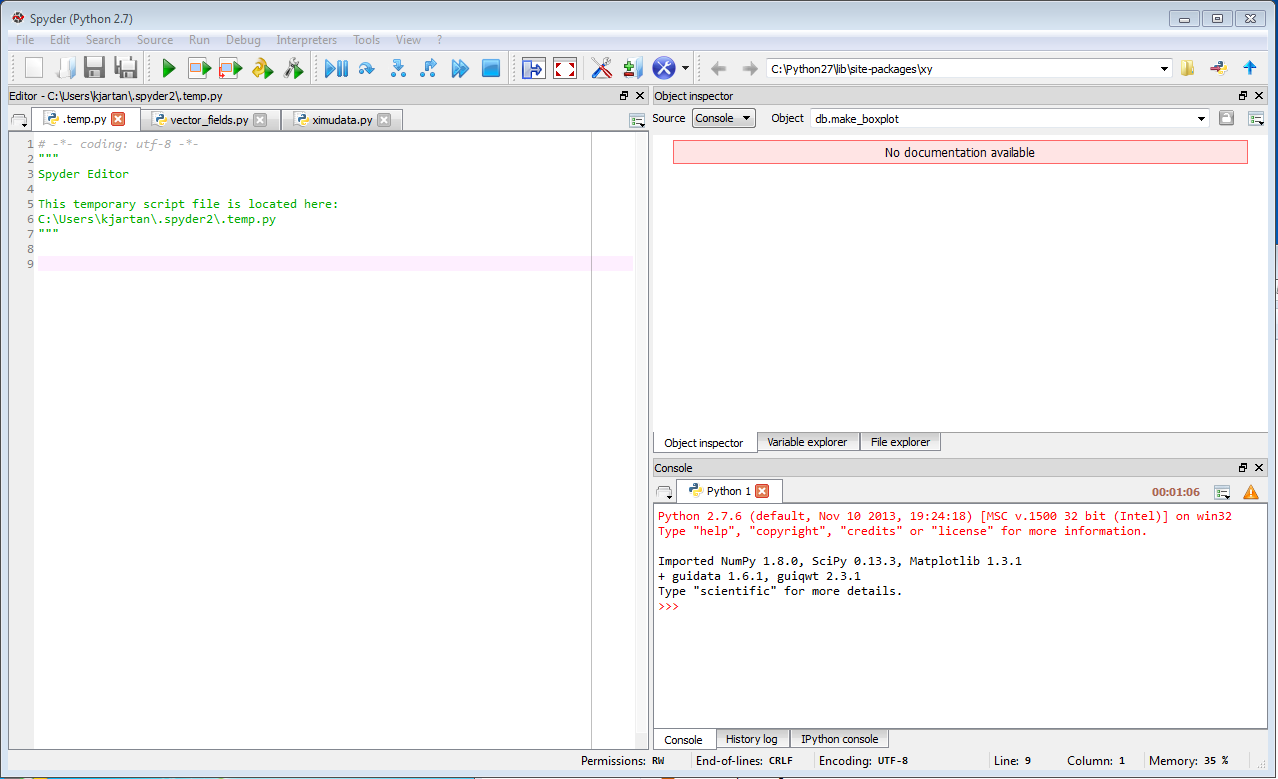
\includegraphics[width=\linewidth]{spyder}
\end{itemize}
\section{Förbereda data}
\label{sec-4}
\begin{itemize}
\item IMU-data måste finnas tillgänglig i csv-format (comma-spaced values). För varje IMU och försöksperson behövs filerna \verb~blabla_CalInertialAndMag.csv~ och \verb~blabla_DateTime.csv~.
\item För att smidigt kunna dela upp filerna i separata försök, så behövs en lista med tidsstämpel när försöken startade. T.ex. en fil \verb~blabla_events.txt~ som ser ut så här
\begin{verbatim}
2013-11-01 20:31:14, b
2013-11-01 20:38:14, m
....
\end{verbatim}
\item I python-filen \verb~imusum/ximu/ximudata.py~ (ca rad 1500) finns en funktion \texttt{nvg\_2012\_09\_data()} som returnerar all nödvändig information om var datafiler ligger för den studien som gjordes september 2012. En motsvarande funktion behöver göras för nya set med data.
\end{itemize}
\section{Lägga till data i databasen}
\label{sec-5}
I \verb~ximudata.py~ görs detta i funktionen \texttt{split\_files\_main} på rad 1450. Först måste databasen öppnas. Sedan läggs data in:
\begin{verbatim}
>>> import imusim.ximu.ximudata as ximudata
>>> db = ximudata.NVGData('/path/to/my/hdf5file.hdf5')
>>> ximudata.split_files_main(db, rawData=nvg_2013_10_data)
\end{verbatim}
Det är viss manuell handpåläggning som måste till för att synkroniseringen ska funka: För varje IMU plottas accelerationen i början av mätfilen. Den dubbla synkroniserings-pulsen borde synas väl. Marker in ett tidsintervall som omfattar pulsen. När detta är gjort för alla IMU'er för försökspersonen, så söks synkroniseringspulsen automatiskt i varje måtfil. Resultatet plottas så att man får en visuell kontroll att algoritmen funkar. Se funktionen \texttt{sync\_signals()}, rad 1260. Enligt dokumentationen för denna:
\begin{verbatim}
Will look for two narrow peaks more than 100 samples but less than
400 samples apart in the list of signals at the given channel.
The first threshold passing is taken as the sync signal.
The packet number and signal index at the peak are returned in a list.
\end{verbatim}

\section{Bearbeta data}
\label{sec-6}
Börja med att ladda in databasen:
\begin{verbatim}
>>> import imusim.ximu.ximudata as ximudata
>>> db = ximudata.NVGData('/path/to/my/hdf5file.hdf5')
\end{verbatim}
Databas-objektet har ett antal metoder (funktioner) som kan anropas för att räkna på data. För att se en lista på dessa
\begin{verbatim}
>>> dir(db)
['__doc__',
 '__init__',
 '__module__',
 'add_imu_data',
 'apply_to_all_trials',
 'close',
 'create_nvg_db',
 'descriptive_statistics_decorator',
 'detect_steps',
 'fix_cycle_events',
 'fname',
 'get_PN_at_sync',
 'get_ROM_joint_angle',
 'get_RoM_angle_to_vertical',
 'get_angle_between_segments',
 'get_angle_to_vertical',
 'get_cycle_data',
 'get_cycle_frequency',
 'get_imu_data',
 'get_minmax_angle_to_vertical',
 'get_minmax_joint_angle',
 'get_orientation',
 'get_range_of_motion',
 'get_trial_attribute',
 'get_vertical_displacement',
 'has_trial_attribute',
 'hdfFile',
 'list_imus',
 'make_boxplot',
 'normalize_statistics',
 'plot_imu_data',
 'track_displacement',
 'track_orientation']
\end{verbatim}
Det första som måste göras är att hitta fotisätningen, så att data kan delas upp i separata gångsteg. Detta görs med metoden \texttt{detect\_steps()}. Ett smidigt sätt om man vill köra denna metoden (eller någon annan metod) på alla försök är att använda metoden \texttt{apply\_to\_all\_trials}:
\begin{verbatim}
>>> db.apply_to_all_trials(db.detect_steps)
\end{verbatim}
För varje försök plottas accelerationen i IMU'en LA (Left Ankle). Kolla på plotten för att bestämma lämplig tröskel. Isätt (start på steg) bestäms som tidpunkt för varje mätpunkt som överstiger tröskeln, givet att det är åtminstone 240 samples sedan förra isättet. Det är alltså en hårdkodad minsta stegduration. Se koden för metoden på rad 302. Resultatet av \texttt{detect\_steps()} lagras i databasen. Man behöver alltså inte göra om detta steget, med mindre det finns anledning att tro att steg-detektionen kunde göras bättre med annat värde på tröskeln.

De flesta beräkningar på data bygger på att man har hittat början på steget, och kan dela upp mätningen i separata steg. Aktuella metoder är 
\begin{verbatim}
'get_ROM_joint_angle',
'get_RoM_angle_to_vertical',
'get_angle_between_segments',
'get_angle_to_vertical',
'get_cycle_data',
'get_cycle_frequency',
'get_minmax_angle_to_vertical',
'get_minmax_joint_angle',
'get_range_of_motion',
'get_vertical_displacement',
\end{verbatim}
Också dess kan anropas på varje försök eller på delmängder av alla försök. T.ex.
\begin{verbatim}
>>> res = db.apply_to_all_trials(db.get_RoM_angle_to_vertical, {'imu':'N'},
                                           subjlist=['S2', 'S3'], triallist=['b', 'n'])
\end{verbatim}
vilket vill beräkna range of motion för vinkeln mot vertikalen för imu N for försöken "b" och "n" för försökspersonerna S2 och S3.
% Emacs 24.5.1 (Org mode 8.2.10)
\end{document}